\documentclass[10pt,letterpaper]{article}
\usepackage[T1]{fontenc}
\usepackage[utf8]{inputenc}
\usepackage{lmodern}
\usepackage[margin=0.77in,headheight=19pt,footskip=26pt]{geometry}
\usepackage{microtype}
\usepackage{parskip}
\usepackage{amsmath,amssymb}
\usepackage{array,tabularx,longtable,booktabs,multirow}
\usepackage[table]{xcolor}
\usepackage{tikz}
\usetikzlibrary{arrows.meta,positioning,shapes.geometric,fit,calc}
\usepackage[most]{tcolorbox}
\usepackage{enumitem}
\usepackage{fancyhdr}
\usepackage{lastpage}
\usepackage{titlesec}
\usepackage{hyperref}
\usepackage{needspace}
\usepackage{ragged2e}
\usepackage{pdflscape}

% --- Color system ---
\definecolor{Ink}{HTML}{14263D}
\definecolor{Navy}{HTML}{142E4C}
\definecolor{Blue}{HTML}{176F9E}
\definecolor{Teal}{HTML}{117C78}
\definecolor{Gold}{HTML}{D59A3B}
\definecolor{PaleBlue}{HTML}{EFF6FA}
\definecolor{PaleTeal}{HTML}{ECF7F4}
\definecolor{PaleGold}{HTML}{FBF5E9}
\definecolor{PaleRed}{HTML}{FCF0ED}
\definecolor{Rule}{HTML}{D7E1E8}
\definecolor{Muted}{HTML}{53677B}
\color{Ink}
\hypersetup{colorlinks=true,linkcolor=Navy,urlcolor=Blue,citecolor=Teal,pdftitle={JAN-PRO of Atlanta | Pre-Purchase Dependency Roadmap},pdfsubject={2026 Atlanta franchise disclosure due diligence},pdfauthor={Franchise Purchase Due-Diligence Guide}}

\setlength{\parindent}{0pt}
\setlength{\parskip}{5pt}
\setlist[itemize]{leftmargin=1.2em,itemsep=2pt,topsep=3pt,parsep=0pt}
\setlist[enumerate]{leftmargin=1.4em,itemsep=2pt,topsep=3pt,parsep=0pt}
\renewcommand{\arraystretch}{1.19}
\titleformat{\section}{\sffamily\bfseries\LARGE\color{Navy}}{\thesection}{.7em}{}
\titleformat{\subsection}{\sffamily\bfseries\large\color{Navy}}{\thesubsection}{.7em}{}
\titleformat{\subsubsection}{\sffamily\bfseries\normalsize\color{Teal}}{\thesubsubsection}{.7em}{}
\titlespacing*{\section}{0pt}{17pt}{9pt}
\titlespacing*{\subsection}{0pt}{13pt}{5pt}

\pagestyle{fancy}
\fancyhf{}
\fancyhead[L]{\scriptsize\sffamily\color{Muted} JAN-PRO OF ATLANTA \quad/\quad PURCHASE DUE DILIGENCE}
\fancyhead[R]{\scriptsize\sffamily\color{Muted} OCTOBER 2026}
\fancyfoot[L]{\scriptsize\color{Muted} Based on the May 1, 2026 FDD \;\textbullet\; Independent review guide}
\fancyfoot[R]{\scriptsize\color{Muted}\thepage\ / \pageref{LastPage}}
\renewcommand{\headrulewidth}{0.5pt}
\renewcommand{\footrulewidth}{0pt}
\renewcommand{\headrule}{\hbox to\headwidth{\color{Rule}\leaders\hrule height \headrulewidth\hfill}}

\newcommand{\FDD}[1]{\textsf{\footnotesize\color{Muted} [FDD: #1]}}
\newcommand{\Link}[2]{\href{#1}{\textcolor{Blue}{#2}}}
\newcommand{\Req}{\textcolor{Navy}{\sffamily\bfseries LEGAL / CONTRACTUAL}}
\newcommand{\Rec}{\textcolor{Teal}{\sffamily\bfseries RECOMMENDED}}
\newcommand{\QBox}{\(\square\)}
\newcolumntype{Y}{>{\RaggedRight\arraybackslash}X}
\newcolumntype{Z}{>{\RaggedLeft\arraybackslash}X}

\tcbset{enhanced,boxrule=.65pt,arc=2.4mm,left=10pt,right=10pt,top=8pt,bottom=8pt,before skip=6pt,after skip=8pt}
\newtcolorbox{prioritybox}[1][]{colback=PaleGold,colframe=Gold,breakable,title={\sffamily\bfseries Decision priority},coltitle=Navy,fonttitle=\sffamily\bfseries,#1}
\newtcolorbox{riskbox}[1][]{colback=PaleRed,colframe=Gold,breakable,title={\sffamily\bfseries Disclosure reconciliation required},coltitle=Navy,#1}
\newtcolorbox{noteBox}[1][]{colback=PaleBlue,colframe=Rule,breakable,#1}
\newtcolorbox{successBox}[1][]{colback=PaleTeal,colframe=Teal,breakable,#1}

\begin{document}
\thispagestyle{empty}
\begin{tikzpicture}[remember picture,overlay]
 \fill[Navy] (current page.north west) rectangle ([yshift=-3.05in]current page.north east);
 \fill[Teal] ([yshift=-3.05in]current page.north west) rectangle ([yshift=-3.15in]current page.north east);
 \fill[Gold] ([xshift=0.76in,yshift=-.72in]current page.north west) rectangle ([xshift=1.78in,yshift=-.77in]current page.north west);
 \draw[white,opacity=.16,line width=2pt] ([xshift=5.2in,yshift=-.47in]current page.north west) -- ([xshift=7.92in,yshift=-2.9in]current page.north west);
 \draw[white,opacity=.16,line width=2pt] ([xshift=6.2in,yshift=-.35in]current page.north west) -- ([xshift=8.3in,yshift=-2.3in]current page.north west);
\end{tikzpicture}
\vspace*{.58in}
{\sffamily\bfseries\color{white}\normalsize 2026 FRANCHISE ACQUISITION REFERENCE}\par
\vspace{.21in}
{\sffamily\bfseries\color{white}\fontsize{30}{36}\selectfont JAN-PRO OF ATLANTA}\par
\vspace{.12in}
{\sffamily\color{white}\fontsize{23}{28}\selectfont Pre-Purchase Dependency Roadmap}\par
\vspace{.17in}
{\sffamily\color{white!85}\large Topological ordering, financial gates, contract risks, and actionable resources}\par
\vspace{1.02in}
{\sffamily\bfseries\color{Navy}\large PURPOSE}\par
A structured pre-purchase decision guide for a prospective unit franchisee of
\textbf{RBJK Marketing, LLC, d/b/a JAN-PRO of Atlanta}. The roadmap orders
critical activities by prerequisite, keeps the \textit{franchise purchase} distinct
from \textit{opening the business}, and converts disclosed risks into verifiable
acceptance criteria.

\begin{noteBox}
\textbf{Primary source:} \emph{Franchise Disclosure Document for Unit Franchises},
RBJK Marketing, LLC, issue date \textbf{May 1, 2026}; supplied file:
\texttt{2026 Atlanta FDD (1)(1).docx}. References to FDD Items and Exhibits
refer to that supplied document. This guide does not replace the controlling
franchise contracts or individualized legal, tax, or financial advice.
\end{noteBox}

\vfill
\begin{tabularx}{\linewidth}{@{}Y Y@{}}
 \textbf{DOCUMENT CLASSIFICATION} & \textbf{PREPARED}\tabularnewline
 Prospective franchisee due diligence & October 10, 2026\tabularnewline
 \textbf{DECISION MILESTONE} & \textbf{PURCHASE RULE}\tabularnewline
 Sign only after dependency gates pass & No premature franchise payment\tabularnewline
\end{tabularx}
\clearpage

\begin{tcolorbox}[colback=PaleBlue,colframe=Rule]
{\sffamily\bfseries\color{Navy}\Large How to use this guide}\par
\textbf{Read the rows in dependency order, not merely numerical order.} Some
branches---document audit, franchisee interviews, and operational feasibility---can
be executed concurrently. A successor may proceed only when its mandatory
predecessors and acceptance evidence are complete.

\vspace{2pt}
\Req{} identifies a requirement stated in the FDD or a government source.
\Rec{} identifies a prudent evaluation step added by this guide, not an
independently established legal obligation.
\end{tcolorbox}
\tableofcontents
\clearpage

\section{Executive decision brief}
\begin{tabularx}{\linewidth}{@{}>{\columncolor{PaleBlue}}p{.28\linewidth}Y@{}}
\toprule
\textbf{Decision variable}&\textbf{Disclosed value and interpretation}\\\midrule
FDD receipt period & At least \textbf{14 calendar days} before a binding franchise agreement or payment to the franchisor or its affiliate in connection with the sale. \FDD{cover; Item 23}\\
Eligible franchisee & An entity (generally LLC or corporation); a sole proprietorship is not permitted. All owners must accept personal obligations. \FDD{Item 1}\\
Initial fees & \$2,000 for the self-acquired-only option; Initial Plan fees range from \$2,520 (discounted) to \$44,000. \FDD{Item 5}\\
Opening investment & FDD cover: \$4,330--\$57,570. The Item 7 table instead states \$4,830--\$58,070 including a California-specific \$500 fee. \FDD{cover; Item 7}\\
Required ongoing royalty & \textbf{10\% of Gross Billings}, not net earnings or collected cash. \FDD{Item 6}\\
Territory & \textbf{Nonexclusive}: competing franchisees or channels may operate in the area. \FDD{Item 12}\\
Term & Initial five years, with two conditional five-year renewals. \FDD{Item 17}\\
Launch timing & FDD describes approximately 45 days from signing to opening, contingent on training and account needs; not a guaranteed deadline. \FDD{Item 11}\\
\bottomrule
\end{tabularx}

\begin{prioritybox}
\textbf{First action:} request a corrected, complete FDD, a reconciliation of
Item 7, substantiation of Item 19, complete executed-agreement templates, and
current/former franchisee references. Do not make a nonrefundable franchise
payment merely to accelerate evaluation.
\end{prioritybox}

\section{Document-integrity and risk review}
\subsection{Disclosure questions that must be resolved}
\begin{tabularx}{\linewidth}{@{}p{.22\linewidth}Y p{.24\linewidth}@{}}
\toprule
\textbf{Issue} & \textbf{What the supplied FDD shows} & \textbf{Evidence to obtain}\\\midrule
Initial-investment discrepancy & Cover: \$4,330--\$57,570. Item 7: \$4,830--\$58,070. Item 7 includes a \$500 California-specific line not applicable to Georgia in the ordinary case. & Corrected Georgia-specific Item 7 table and estimate assumptions.\\
Financial-performance omission & Item 19's two-franchisee performance example table is unpopulated. Its \emph{100\% compliance} assertion addresses account-offering obligations, not profitability. & Completed/clarified Item 19 and substantiation for the stated account-offering compliance.\\
Outlet movement & Item 20 lists 444 Georgia unit outlets at the end of 2024 and 437 at the end of 2025. For 2025, it lists 71 openings, 5 terminations, 25 nonrenewals, and 48 other cessation events. & Explanations of nonrenewals, cessation categories, account economics, and operator experiences.\\
Additional-account fee illustrations & Item 6 describes 4\(\times\) monthly billings below \$20,000 annualized billings and 3\(\times\) at or above it; adjacent examples of \$200/month imply \$1,000 and \$800 rather than the resulting \$800 and \$600. & Written corrected fee examples and calculation policy.\\
Drafting defects & Item 11 includes an unfilled trainer placeholder; Item 21 describes ``September 31st, 2026,'' a nonexistent date. & Updated FDD or specific explanation of discrepancies and signed documents.\\
\bottomrule
\end{tabularx}

\begin{riskbox}
A discrepancy is a \emph{verification issue}, not proof of misconduct. The FDD's
figures are reproduced as stated and the conflicts identified explicitly; none
is silently treated as corrected. Ask counsel which changes require delivery of
an updated disclosure and whether additional review time applies.
\end{riskbox}

\section{Dependency architecture}
\subsection{Critical purchase path}
\begin{figure}[htbp]
\centering
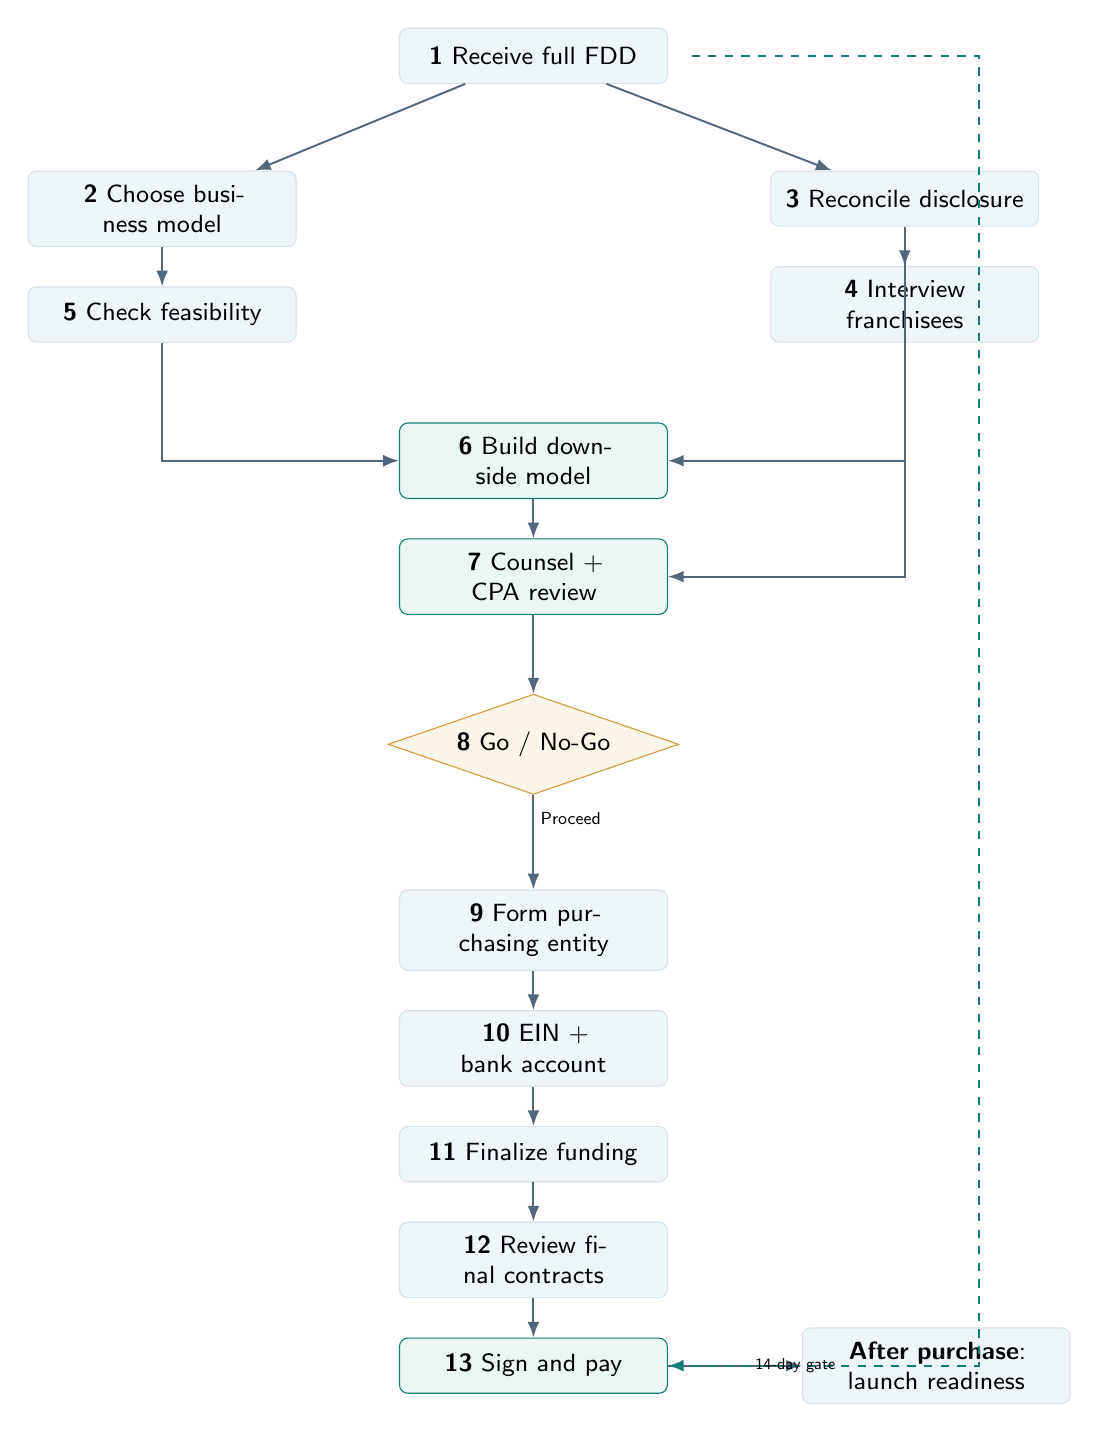
\begin{tikzpicture}[
    font=\sffamily\small,
    node distance=5mm and 10mm,
    task/.style={draw=Rule,fill=PaleBlue,rounded corners=3pt,text width=3.05cm,align=center,minimum height=.7cm,inner sep=5pt},
    check/.style={draw=Teal,fill=PaleTeal,rounded corners=3pt,text width=3.05cm,align=center,minimum height=.7cm,inner sep=5pt},
    decision/.style={draw=Gold,fill=PaleGold,diamond,aspect=2.9,text width=2.5cm,align=center,inner sep=1pt},
    arr/.style={-{Latex[length=2.0mm]},line width=.7pt,draw=Muted}]
\node[task] (a) {\textbf{1} Receive full FDD};
\node[task,below left=11mm and 13mm of a] (b) {\textbf{2} Choose business model};
\node[task,below right=11mm and 13mm of a] (c) {\textbf{3} Reconcile disclosure};
\node[task,below=of b] (e) {\textbf{5} Check feasibility};
\node[task,below=of c] (d) {\textbf{4} Interview franchisees};
\node[check,below=17mm of a,yshift=-26mm] (f) {\textbf{6} Build downside model};
\node[check,below=of f] (g) {\textbf{7} Counsel + CPA review};
\node[decision,below=10mm of g] (h) {\textbf{8} Go / No-Go};
\node[task,below=12mm of h] (i) {\textbf{9} Form purchasing entity};
\node[task,below=of i] (j) {\textbf{10} EIN + bank account};
\node[task,below=of j] (k) {\textbf{11} Finalize funding};
\node[task,below=of k] (l) {\textbf{12} Review final contracts};
\node[check,below=of l] (m) {\textbf{13} Sign and pay};
\node[task,right=17mm of m] (n) {\textbf{After purchase}: launch readiness};
\draw[arr] (a) -- (b); \draw[arr] (a) -- (c);
\draw[arr] (b)--(e); \draw[arr] (c)--(d);
\draw[arr] (e) |- (f); \draw[arr] (d) |- (f);
\draw[arr] (f)--(g);\draw[arr] (c) |- (g);
\draw[arr] (g)--(h); \draw[arr] (h)--node[right,near start,scale=.7]{Proceed}(i);
\draw[arr] (i)--(j);\draw[arr] (j)--(k);\draw[arr] (k)--(l);\draw[arr] (l)--(m);\draw[arr] (m)--(n);
\draw[arr,dashed,draw=Teal] ([xshift=3mm]a.east) -- ++(3.65cm,0) |- node[pos=.87,right,scale=.64]{14-day gate} ([xshift=0mm]m.east);
\end{tikzpicture}
\caption{High-level dependency graph. Financial analysis also depends on the proposed business model and independent operator feedback; the dependency register below is authoritative where diagram routing is simplified.}
\end{figure}

\subsection{Ordered dependency register}
{\small
\begin{longtable}{@{}p{.08\linewidth}p{.245\linewidth}p{.13\linewidth}p{.44\linewidth}@{}}
\toprule
\textbf{ID} & \textbf{Activity} & \textbf{Prerequisite} & \textbf{Evidence of completion}\\\midrule
\endfirsthead
\toprule\textbf{ID}&\textbf{Activity}&\textbf{Prerequisite}&\textbf{Evidence of completion}\\\midrule
\endhead
1 & Receive and date complete FDD & None & Receipt date and full document/exhibit inventory preserved.\\
2 & Select ownership and purchase model & 1 & Initial Plan vs. self-acquired accounts; staffing and support choices recorded.\\
3 & Reconcile disclosures & 1 & Material inconsistencies answered in writing; updated documents as necessary.\\
4 & Interview franchisees & 1 & Current/former operator interview notes and corroborating evidence.\\
5 & Validate local feasibility & 2 & Service-area, capacity, staffing, licensing, equipment, and insurance plan.\\
6 & Model profitability and liquidity & 2, 4, 5 & Base/downside cash model; no reliance on estimated billings as profits.\\
7 & Attorney/CPA due diligence & 3, 6 & Contract exceptions and financial/tax assessment signed off.\\
8 & Conditional Go/No-Go & 4, 6, 7 & Written decision with unresolved risk list and maximum loss tolerance.\\
9 & Form Georgia entity & 8 (go) & Georgia entity record and ownership structure.\\
10 & Obtain EIN; establish bank account & 9 & EIN confirmation and dedicated business banking.\\
11 & Finalize capital and readiness plan & 6, 8, 9 & Funding terms, liquidity reserve, quotes, permit and training schedule.\\
12 & Review fully completed documents & 7, 9, 11 & Final franchise terms, finance note, guarantees, and optional services checked.\\
13 & Sign and make payment & 12, 14-day gate & All applicable review periods satisfied; executed copies and payment records.\\
\bottomrule
\end{longtable}}

\section{Execution playbook: before signing}
\subsection{Stage A --- disclose, choose, investigate (steps 1--5)}
\textbf{Step 1: Receive the FDD.} Record the actual day of delivery, retain the
receipt and the entire delivered package, confirm all 23 items and exhibits,
and calculate the earliest permissible franchise signing/payment date. In the
usual federal framework, the FDD must be delivered at least 14 calendar days
before the prospective purchaser signs or pays. Any separate final-agreement
review rule must be evaluated by counsel. \FDD{cover; Item 23}

\textbf{Step 2: Choose the business model.} Decide between the \$2,000
self-acquired-only initial fee and a purchased Initial Plan; select a proposed
annual account-billings tier, a staffing approach, service geography, and
which of three optional support programs, if any, are economically desirable.
\FDD{Items 1, 5--6, 11}

\textbf{Step 3: Reconcile the FDD.} Obtain written answers on the inconsistent
investment table, incomplete Item 19 figures, 2025 outlet departures, fee
examples, and incomplete administrative disclosures. Review franchisor
litigation and financial statements rather than relying on sales presentations.
\FDD{Items 3--4, 6--7, 19--21}

\textbf{Step 4: Interview operators.} Contact a diverse sample of current and
former unit franchisees from the disclosed lists. Ask for ranges for actual
collected revenue, labor hours, drive time, customer retention, nonpayment,
fee deductions, equipment replacement, and exit costs. Request documents
where operators voluntarily provide them; honor confidentiality obligations.
\FDD{Item 20; Exhibits E--F}

\textbf{Step 5: Establish operational feasibility.} Verify whether you can
reliably service candidate customer schedules and locations, including evening
work, travel, access requirements, staff availability, chemical safety,
specialized cleaning, insurance, and licensing in the actual place of business.
Do not assume JAN-PRO's Marietta headquarters determines your local license
jurisdiction. \FDD{Items 7--8, 11--12}

\subsection{Stage B --- underwrite and approve (steps 6--8)}
\textbf{Step 6: Underwrite cash flow.} For each viable plan, build a 12-month
monthly forecast (and a three-year view, where feasible) that separates
\emph{accounts offered}, \emph{accounts activated}, \emph{invoices sent}, and
\emph{cash received}. Test delayed start dates, unfilled plan volume, customer
churn, delinquency, staffing shortages, and unexpected equipment costs. Compare
all-cash, franchisor-financed, and self-acquired-account strategies.

\textbf{Step 7: Obtain independent reviews.} Retain a Georgia lawyer with
franchise-transaction experience to review the agreement, promissory note,
personal guarantees, collateral, account repossession, termination, noncompete,
renewal, transfer, and dispute resolution. Have a CPA review audited statements,
working capital, payroll taxes, entity elections, and tax assumptions.

\textbf{Step 8: Decide.} Record the decision, acceptable purchase ceiling,
minimum liquidity reserve, and the risks accepted or still outstanding. A
\emph{Go} decision is conditional on obtaining acceptable, complete transaction
documents and realistic funding. A \emph{No-Go} decision ends the transaction
before significant sunk operating costs.

\subsection{Stage C --- establish purchaser and close (steps 9--13)}
\textbf{Step 9: Form the purchasing entity.} An LLC or corporation must serve as
the unit franchisee; the FDD excludes sole proprietorship. Consider ownership,
registered-agent arrangements, operating agreement, and the effect of mandatory
owner guarantees. Form using the \Link{https://sos.ga.gov/how-to-guide/how-guide-register-domestic-entity}{Georgia Secretary of State's domestic-entity guide}. \FDD{Item 1}

\textbf{Step 10: Complete tax/banking setup.} Obtain the free EIN directly from
\Link{https://www.irs.gov/businesses/small-businesses-self-employed/get-an-employer-identification-number}{the IRS} and establish dedicated business banking. Determine any separate
Georgia state tax and employer registrations.

\textbf{Step 11: Finalize financial capacity.} Confirm precise initial fee,
franchisor financing terms (if elected), down payment, interest, repayment
schedule, restricted cash, emergency reserve, required insurance, likely wages,
and the expense of reaching the defined Start Date. Do not treat approval for
a 10\% financed fee balance as evidence that the business is viable. \FDD{Items 5, 7, 10}

\textbf{Step 12: Review \emph{completed} final agreements.} Match legal names,
plan, billed-volume tier, exhibits, guarantors, payment and security documents,
program opt-ins, termination language, and written clarifications. Confirm with
counsel whether a new contract revision triggers an additional review period.
\FDD{Item 22; Exhibits A--B}

\textbf{Step 13: Sign and pay.} Execute the agreed documents only after the
required disclosure/review periods, entity formation, due diligence, and final
risk acceptance. Preserve the signed franchise agreement, note, program
elections, FDD receipt, invoice, and bank record.

\section{Franchise fees and account economics}
\subsection{Representative Initial Plan comparison}
\begin{table}[htbp]
\centering\small
\begin{tabularx}{\linewidth}{@{}l r r r r@{}}
\toprule
\textbf{Plan} & \textbf{Annual account billings\textsuperscript{a}} & \textbf{All-cash fee} & \textbf{Financed down} & \textbf{Balance financed}\\\midrule
FP-5 & \$5,000 & \$2,520 & \$950 & \$1,850\\
FP-20 & \$20,000 & \$8,100 & \$5,000 & \$4,000\\
FP-50 & \$50,000 & \$14,400 & \$11,000 & \$5,000\\
FP-100 & \$100,000 & \$23,400 & \$21,000 & \$5,000\\
FP-200 & \$200,000 & \$39,600 & \$36,500 & \$7,500\\
\bottomrule
\end{tabularx}
\caption{Selected values from FDD Item 5. \textsuperscript{a}\emph{Estimates} of annual gross billings for accounts offered under a plan; not guarantees of collections, income, or profit. All-cash fees reflect the stated 10\% discount. Financing carries 10\% annual interest under disclosed terms.}
\end{table}

\subsection{Ongoing and contingent charge schedule}
{\small
\begin{tabularx}{\linewidth}{@{}p{.265\linewidth}p{.21\linewidth}Y@{}}
\toprule
\textbf{Charge} & \textbf{Disclosed amount} & \textbf{When to account for it}\\\midrule
Royalty & 10\% of Gross Billings & Required monthly; gross-billings basis differs from cash receipts.\\
Support Services Program & 5\% of Gross Billings & Optional monthly billing/collection program.\\
Advance Assurance & 2\% of Gross Billings & Optional receivables protection program with contractual limitations.\\
Business Protection Program & Currently 6\% of Gross Billings & Optional; fee may change with insurance cost.\\
National Account Support & Additional 2\% & Qualifying national-account Gross Billings.\\
Special Services administration & Additional 10\% & Gross Billings from qualifying nonrecurring services.\\
Technology fee & Up to \$60 monthly & If imposed, per Item 6.\\
Additional referred account & 4\(\times\) or 3\(\times\) monthly account billings & 4\(\times\) below \$20k in franchisee annualized billings; 3\(\times\) at/above. Verify the FDD's inconsistent worked examples.\\
Renewal & \$750 & Before approved renewal.\\
Business transfer & Greater of \$1,500 or 8\% of trailing 12-month Gross Billings & Before a permitted transfer.\\
\bottomrule
\end{tabularx}}
\FDD{Items 5--6, 17; Support Services Agreement}

\begin{noteBox}
\textbf{Illustrative fee stack:} 10\% standard royalty + 5\% support + 2\%
Advance Assurance + 6\% Business Protection = \textbf{23\% of Gross
Billings}, at disclosed current rates, if all three optional programs are
selected. This excludes labor, supplies, travel, taxes, financing, and any
other triggered fees. The example is not a recommendation to enroll in every
program.
\end{noteBox}

\subsection{Monthly cash-flow worksheet and decision tests}
\begin{align*}
\text{Net operating cash flow}_t={}&\text{Customer cash received}_t\\
&-\text{Franchisor / support fees}_t\\
&-\text{Wages, taxes, and labor overhead}_t\\
&-\text{Supplies, transport, insurance, overhead}_t\\
&-\text{Debt service and capital outlays}_t.
\end{align*}
\textbf{Model explicitly:} (i) estimated annual account billings vs. realized
monthly amounts; (ii) onboarding delays and phased delivery of accounts;
(iii) billing-to-collection lag; (iv) owner replacement labor and payroll
burden; (v) loss/replacement of accounts; (vi) finance payments and guaranty
exposure; and (vii) a minimum liquidity threshold.

\begin{tabularx}{\linewidth}{@{}p{.21\linewidth}Y Y@{}}
\toprule
\textbf{Scenario} & \textbf{Operating assumption} & \textbf{Decision question}\\\midrule
Base & Expected staffing, account acceptance, retention, and receipts & Is net cash positive \emph{after} fees and an owner labor allowance?\\
Downside & Slower account delivery, higher wage/route burden, collection delays & Can available cash cover obligations with no new borrowing?\\
Severe downside & Material customer loss and several months' low utilization & What is the maximum committed loss, including guaranties?\\
\bottomrule
\end{tabularx}

\begin{riskbox}
Item 7's stated three-month ``additional funds'' allowance excludes several
major potential expenditures, including owner compensation, royalties, other
amounts due to the franchisor, and replacement supplies. Develop an
independent working-capital budget; do not assume the FDD estimate is a
complete operating reserve. \FDD{Item 7, Note 12}
\end{riskbox}

\subsection{Account-delivery constraints}
The franchisor generally has \textbf{120 business days after the contractual
Start Date} to offer an Initial Plan's required account billings. For an
Initial Plan above \$35,000, Item 5 adds \textbf{30 business days per \$15,000
or portion thereof} above \$35,000, subject to stated extensions. For
FP-200, the unextended formula is:
\[
120+30\left\lceil \frac{200{,}000-35{,}000}{15{,}000}\right\rceil
=\boxed{450\text{ business days}.}
\]
The formula concerns the \emph{time to offer account volume}, not a
promise of collections or profit. Ask what constitutes a qualified offer,
what happens after rejection, and how substitutions/refunds actually operate.
\FDD{Item 5: Our Time to Fulfill the Initial Plan}

\section{Attorney and franchisee interview matrix}
{\small
\begin{longtable}{@{}p{.23\linewidth}p{.58\linewidth}p{.14\linewidth}@{}}
\toprule
\textbf{Topic} & \textbf{Question to resolve in writing} & \textbf{FDD source}\\\midrule
\endfirsthead
\toprule\textbf{Topic}&\textbf{Question to resolve in writing}&\textbf{FDD source}\\\midrule\endhead
Guaranties & Which obligations extend personally to owners and any spouse; what is the maximum realistic exposure? & Cover risk disclosures; Items 1, 10\\
Financing / collateral & What liens cover equipment, receivables, contracts and future franchise assets? What triggers default? & Items 5, 10; note\\
Territory & Which accounts/locations are permitted and what does nonexclusivity mean operationally? & Item 12\\
Pricing / labor hours & Can the purchaser inspect bid worksheets, contracted frequency, site conditions, service hours, and wage assumptions before account acceptance? & Cover special risks; Items 5--6\\
Account retention & Under what events may accounts be repossessed or reassigned? When do replacement rights end? & Item 5; franchise agreement\\
Payment risk & How are delinquent customer accounts treated under each optional billing/advance arrangement? & Items 5--6; support agreement\\
Exit & Are early termination rights limited? What amounts, guarantees, noncompetes, and transfer conditions survive termination? & Item 17\\
Document inconsistencies & Which amended FDD or correction letter resolves the uncovered omissions and miscalculations? & Items 6--7, 11, 19, 21\\
\bottomrule
\end{longtable}}

\begin{successBox}
\textbf{Operator evidence target:} discuss pricing and account economics with
both profitable and unsuccessful former/current franchisees. The provided Item
19 statement that account-offering obligations were satisfied in 100\% of 68
sales during 2025 is \emph{not} a franchisee-profitability statistic.
\end{successBox}

\section{Business readiness after signing}
\textbf{Do not confuse prerequisites to purchase with prerequisites to
commence operations.} The FDD's \emph{Start Date} depends on:
\begin{enumerate}
 \item Required licenses and permits for the purchasing entity;
 \item The required initial equipment/supplies package;
 \item Required insurance;
 \item Completion of the JAN-PRO Certification Program; and
 \item Other reasonable conditions required by the franchisor.
\end{enumerate}
\FDD{Item 5: Start Date; Item 11}

The FDD describes \textbf{22 classroom hours} of initial certification,
with web-enabled or office-based training, and typically about \textbf{45 days}
from agreement signing to business opening. Confirm scheduling and any account-
specific advanced certification before purchasing. \FDD{Item 11}

\begin{tabularx}{\linewidth}{@{}p{.245\linewidth}Y@{}}
\toprule
\textbf{Workstream} & \textbf{Official resource (clickable)}\\\midrule
Georgia entity formation & \Link{https://sos.ga.gov/how-to-guide/how-guide-register-domestic-entity}{Georgia Secretary of State: Register a domestic entity}\\
Federal EIN & \Link{https://www.irs.gov/businesses/small-businesses-self-employed/get-an-employer-identification-number}{IRS: Obtain an EIN at no charge}\\
Georgia state tax & \Link{https://dor.georgia.gov/taxes/register-new-business-georgia}{Georgia Department of Revenue: Register a new business}\\
Georgia employer setup & \Link{https://georgia.gov/register-business-georgia-department-labor}{Georgia Department of Labor: Business registration}\\
Local occupational license & \Link{https://www.cobbcounty.gov/community-development/business-license/obtain-business-license}{Cobb County business licenses}; \Link{https://www.atlantaga.gov/government/departments/finance/office-of-revenue/apply-for-a-new-business-occupational-tax-certificate}{City of Atlanta occupational tax certificate}\\
Workers' compensation & \Link{https://sbwc.georgia.gov/employer-information}{Georgia State Board of Workers' Compensation: Employers}\\
Cleaning safety & \Link{https://www.osha.gov/cleaning-industry/hazards-solutions}{OSHA: Cleaning industry hazards}; \Link{https://www.osha.gov/laws-regs/regulations/standardnumber/1910/1910.1200}{Hazard Communication (29 CFR 1910.1200)}\\
\bottomrule
\end{tabularx}

\section{Source map and reference URLs}
\subsection{FDD navigation}
\begin{tabularx}{\linewidth}{@{}p{.29\linewidth}Y@{}}
\toprule
\textbf{Topic} & \textbf{Read these sections of the supplied 2026 Atlanta FDD}\\\midrule
Purchase fees and financing & Items 5, 6, 7, 10; Franchise Agreement and Promissory Note\\
Support, training and supplies & Items 8, 9, 11, 15; Support Services Agreement\\
Geography and customer rights & Items 5, 12, 16; Franchise Agreement\\
Litigation and financial health & Items 1--4, 19, 20, 21; audited statements, outlet lists\\
Term, renewal, termination & Item 17; Franchise Agreement\\
Contracts and disclosure waiting period & Items 22--23; exhibits and receipt\\
\bottomrule
\end{tabularx}

\subsection{Federal franchise guidance}
\begin{itemize}
\item \Link{https://www.ftc.gov/business-guidance/resources/consumers-guide-buying-franchise}{FTC --- A Consumer's Guide to Buying a Franchise}.
\item \Link{https://www.ftc.gov/business-guidance/resources/amended-franchise-rule-faqs}{FTC --- Amended Franchise Rule FAQs}, including disclosure and completed agreement review questions.
\item \Link{https://georgia.gov/starting-business-guide}{Georgia.gov --- Starting a Business Guide}.
\end{itemize}

\begin{noteBox}
\textbf{Source discipline.} FDD-derived facts are identified by Item/Exhibit;
external agency links are provided for procedural research and may change.
Independent analytical recommendations (scenario testing, interview structure,
and go/no-go thresholds) are not assurances made by JAN-PRO. Confirm current
fees, requirements, and jurisdiction directly with the appropriate authorities.
\end{noteBox}

\clearpage
\section{Go/No-Go decision card}
\begin{noteBox}
Complete this printable review page only after the upstream dependencies have been evaluated. Retain it with the final investment memorandum.
\end{noteBox}
\begin{tcolorbox}[colback=white,colframe=Teal,title={\sffamily\bfseries PURCHASE GATE --- PRINT / COMPLETE}]
\begin{tabularx}{\linewidth}{@{}p{.09\linewidth}Y@{}}
\QBox & Complete FDD, agreements, exhibits, and receipt date retained.\\[4pt]
\QBox & Item 7, Item 19, fees, and other material inconsistencies addressed.\\[4pt]
\QBox & Current and former franchisees independently interviewed.\\[4pt]
\QBox & Proposed plan, geographic capacity, staffing, and customer requirements evaluated.\\[4pt]
\QBox & Fee-adjusted forecast and severe-downside working-capital scenario reviewed.\\[4pt]
\QBox & Attorney reviewed guarantees, collateral, accounts, exit, and noncompete terms.\\[4pt]
\QBox & CPA reviewed tax structure, costs, and franchisor financial statements.\\[4pt]
\QBox & Explicit Go/No-Go decision documented; financing and liquidity secured.\\[4pt]
\QBox & Purchasing entity and EIN established; bank account available.\\[4pt]
\QBox & Final contracts reviewed; all applicable disclosure waiting periods elapsed.\\
\end{tabularx}
\tcblower
\textbf{Decision:} \QBox\ GO \qquad \QBox\ NO-GO \qquad \QBox\ DEFER / REQUEST INFORMATION

\vspace{8pt}
\noindent\textbf{Approved budget:} \rule{1.30in}{.4pt}\hfill
\textbf{Minimum liquidity:} \rule{1.35in}{.4pt}

\vspace{10pt}
\textbf{Outstanding conditions:} \rule{4.65in}{.4pt}

\vspace{16pt}
\textbf{Reviewer:} \rule{2.5in}{.4pt}\qquad
\textbf{Date:} \rule{1.65in}{.4pt}
\end{tcolorbox}


\subsection*{Decision notes and approval conditions}
\textit{Record material risks, agreed mitigations, and outstanding evidence.}

\vspace{13pt}\noindent\rule{\linewidth}{.3pt}

\vspace{13pt}\noindent\rule{\linewidth}{.3pt}

\vspace{13pt}\noindent\rule{\linewidth}{.3pt}

\vspace{13pt}\noindent\rule{\linewidth}{.3pt}

\vspace{13pt}\noindent\rule{\linewidth}{.3pt}
\vfill
{\centering\sffamily\bfseries\color{Navy} END OF PRE-PURCHASE ROADMAP\par}
\end{document}
